%% \chapter[htoc-titlei][hhead-titlei]{htitlei}
%% -----------------------------------------------------------------------------
\chapter[Theoretical Framework][Theoretical Framework]{Theoretical Framework} \label{ch:theory}

In this chapter the mathematical theoretical framework is presented in which the physical measurements and computational modeling will be interpreted in the subsequent chapters.
For elementary particle physics this framework is \gls{qft}, a relativistically consistent quantum mechanics who's fundamental mathematical objects are fields instead of particles.
Within the mathematical umbrella of QFT comes one of the most successful physical theories ever developed, the Standard Model (SM) of particle physics.
While the success of the SM is undisputed, in its current form it can give no explanation for several big questions in physics. 
This invariably leads to extensions to the SM, known as beyond the the standard model (BSM) physics, with one of the most important and attractive extensions known as Supersymmetry.

%Composed of \gls{qed}, a QFT that describes the  interaction, and \gls{qcd}, a QFT that describes the strong interaction, the SM 

\section{Quantum Field Theory} \label{sec:qft}

\chapter[Formulation of QFT][Formulation of QFT]{Formulation of QFT}
\section{Formulation of QFT}\label{app:qft}
I find it easiest, and maybe the most logically satisfying, to think of the formulation of QFT in terms of canonical quantization (or second quantization). 
Whereby the idea here is to retain the familiar form of the classical Hamiltonian (or Langrangian) representation and then leap from a classical theory to a quantum one by promoting fundamental measurables of physical objects to operators and Poisson brackets to commutators.
So more explicitly the steps are 
\begin{enumerate}
    \item Assume the quantum field Hamiltonian density has the same form as the classical field Hamiltonian density
    \item Replace the classical Poisson brackets for conjugate property densities with commutator brackets (divided by i$\hbar$), i.e.
    $A\rightarrow \hat{A}, \hspace{0.2cm} \{A,B\} \rightarrow\frac{1}{i\hbar}[\hat{A},\hat{B}]$, where the ``hatting'' of the variables signifies the the classical field dynamical variables becoming quantum field non-commuting operators as a consequence of this imposition.
\end{enumerate}
As an example we wlll quantize the most basic resulting QFT, scalar field theory. 
The classical scalar field, $\phi(x,t)$, takes in the position and time and produces the value of the field at that position and time.
Classically, a scalar field is a collection of an infinity of oscillator normal modes.
So the classical Lagrangian density describing an infinite number of coupled harmonic oscillators is written as
\begin{equation}
    \mathcal{L}(\phi)= \frac{1}{2}(\partial_{t}\phi)^2 - \frac{1}{2}(\partial_{x}\phi)^2 - \frac{1}{2}m^{2}\phi^{2} - V(\phi)
\end{equation}
Where $V(\phi)$ is a potential term.
The action is then,
\begin{equation*}
    S(\phi)= \int \mathcal{L}(\phi)dxdt = \int L(\phi, \partial_{t}\phi)dt
\end{equation*}
The canonical momentum can be obtained from the action via the Legendre transformation, and is is found to be  $\displaystyle \pi =\partial _{t}\phi$.
The classical Hamiltonian is then,
\begin{equation}
    H(\phi,\pi) = \int dx\left[ \frac{1}{2}\pi^2 + \frac{1}{2}(\partial_{x}\phi)^2 + \frac{1}{2}m^{2}\phi^{2} + V(\phi) \right]
    \label{eq:theory:hammy}
\end{equation}
Next we impose the canonical commutation relations at $t$=0 as follows
\begin{equation*}
 [\phi(x),\phi(y)] = 0,  \hspace{0.5cm} [\pi(x), \pi(y)] = 0, \hspace{0.5cm} [\phi(x),\pi(y)] = i\hbar \delta(x-y)
\end{equation*}
The operators can then be generalized to and time $t$ in the future by applying the time evolution operator $\mathcal{O}$,
\begin{equation*}
     \mathcal{O}(t) = e^{itH} \mathcal{O} e^{-itH} .
\end{equation*}
Where at this point a choice of $V(\phi)$ is required.
For simplicity we will just consider the case of the free field with $V(\phi)$=0.
It is useful to Fourier transform the fields,
\begin{equation*}
      \phi_k = \int \phi(x) e^{-ikx} dx, \hspace{0.5cm} \pi_k = \int \pi(x) e^{-ikx} dx .
\end{equation*}
It can then be identified that,
\begin{equation*}
    \phi_{-k} = \phi_k^\dagger, \hspace{0.5cm} \pi_{-k} = \pi_k^\dagger.
\end{equation*}
Expanding the Hamiltonian density in Equation~\ref{eq:theory:hammy} in Fourier modes,
\begin{equation}
     H=\frac{1}{2}\sum_{k=-\infty}^{\infty}\left[\pi_k \pi_k^\dagger + \omega_k^2\phi_k\phi_k^\dagger\right],
     \label{eq:theory:quantumhammy}
\end{equation}
where $ {\displaystyle \omega _{k}={\sqrt {k^{2}+m^{2}}}}\omega_k = \sqrt{k^2+m^2}$.
We recognize this Hamiltonian as an infinite sum of classical oscillators $\phi_{k}$, each one of which is quantized in the standard manner, so the free quantum Hamiltonian looks identical. It is the $\phi_{k}$s that have become operators obeying the standard commutation relations, $[\phi_{k},\pi_{k}^{\dagger}] = [\pi_{k}^{\dagger},\phi_{k}] = i\hbar$  with all others vanishing.
The Hilbert space of all these oscillators is constructed using creation and annihilation operators determined from these modes,
\begin{equation*}
     a_k = \frac{1}{\sqrt{2\hbar\omega_k}}\left(\omega_k\phi_k + i\pi_k\right), \ \ a_k^\dagger = \frac{1}{\sqrt{2\hbar\omega_k}}\left(\omega_k\phi_k^\dagger - i\pi_k^\dagger\right), 
\end{equation*}
Subtracting of the zero-point energy $\hbar\omega_{k}/2$ from the Hamiltonian in Equation~\ref{eq:theory:quantumhammy} in order to satisfy the condition that $H$ must annihilate the vacuum and rewriting in terms of the creation/annihilation operators teh Hamiltonian takes the form,
\begin{equation}
     H = \sum_{k=-\infty}^{\infty} \hbar\omega_k a_k^\dagger a_k = \sum_{k=-\infty}^{\infty} \hbar\omega_k N_k
\end{equation}
where $N_k$ may be interpreted as the number operator giving the number of particles in a state with momentum $k$.
% Would like to put a few example Lagrangians of other theories (phi 4 , complex scalar,, and ) with brief qualitative descriptions 
Now, commutation relations are useful only for quantizing bosons, for which the occupancy number of any state is unlimited. To quantize fermions, which satisfy the Pauli exclusion principle, anti-commutators are needed. i.e. the relation  \{A,B\} = AB+BA.
When quantizing fermions, the fields are expanded into the creation and annihilation operators, $b_{k}^{\dagger}$, $b_{k}$, which satisfy
\begin{equation}
    \{ b_{k}, b_{l}^{\dagger}\} = \delta_{k,l}, ~  \{ b_{k}, b_{l}\} = 0, ~ \{ b_{k}^{\dagger}, b_{l}^{\dagger}\} = 0
\end{equation}

All other fields can be quantized by a generalization of this procedure. Vector or tensor fields simply have more components, and independent creation and destruction operators must be introduced for each independent component. If a field has any internal symmetry, then creation and destruction operators must be introduced for each component of the field related to this symmetry as well. If there is a gauge symmetry, then the number of independent components of the field must be carefully analyzed to avoid over-counting equivalent configurations, and gauge-fixing may be applied if needed~\cite{2013.Klauber}.



%begin{equation}
%Q_{\{f,g\}}=\frac{1}{i\hbar}[Q_{f},Q_{g}]
%\label{eq:qft}
%\end{equation}


\section{The Standard Model} \label{sec:sm}
%\textcolor{red}{\hrulefill \textsc{Unfinished Section}\hrulefill}  \\
\begin{figure}
    \centering
    \includegraphics[width=0.90\textwidth]{figs/theory/Standard_Model_Of_Particle_Physics--Most_Complete_Diagram.png}
    \caption[Particle content of the Standard Model both before and after spontaneous symmetry breaking.
    Also shown is an illustration of spontaneous symmetry breaking via the Higgs Mechanism]{Particle content of the Standard Model both before and after spontaneous symmetry breaking.
    Also shown is an illustration of spontaneous symmetry breaking via the Higgs Mechanism~\cite{wiki:xxx}}
    \label{fig:theory:SM}
\end{figure}
Modern particle physics is generally interpreted in terms of the Standard Model (SM).
The SM is a QFT which encapsulates our understanding of the electromagnetic, weak, and strong interactions.
Noticeably missing of course is the force of gravity, which is described by Einstein's General Relativity (GR). 
Theories that reconcile GR and QFT belong to a topic that would take up it's own library and shall not be discussed further as Gravity is so comparably small for our experiments in particle physics that it has no measurable effect and can be easily ignored.
The SM obeys a set of symmetries such that the theory belongs the gauge unitary product group 
\begin{equation}
    SU(3)_{C} \times SU(2)_{L} \times U(1)_{Y}
\end{equation}

\subsection{Quantum Chromodynamics}\label{sec:theory:QCD}
$SU(3)_{C}$ is the gauge symmetry group for the theory of the strong force, Quantum Chromodynamics (QCD), which defines the strong interaction between quarks and gluons.
The strong force is mediated by the force carrying gluons, which each carry the color charges (red, green, blue) and anti-color charges (anti-red, anti-green, anti-blue), leading to a total of 9 possible states of gluons.
However the special color singlet state, which would be indicative of a long range force like the photon, is not observed in nature and so only 8 physical color states are possible.
Gluon-gluon interactions constrain the color fields to string-like objects called ``flux tubes'', so that as two quarks are pulled apart there is a binding energy that increases linearly with their separation.
At a large enough distance, it becomes energetically more favorable to pull a quark-antiquark pair out of the vacuum rather than increase the length of the flux tube.
A phenomenon known as color confinement, this has a cascading effect of the two very energetically separating quarks pulling quark-antiquark pairs out of the vacuum along their journey (which also in turn can do the same), thereby forming hadrons is known as hadronization.
This is an experimentally confirmed phenomenon showing up in particle detectors as large conical sprays or \emph{jets} of particles.

\subsection{Electroweak Unification}\label{sec:theory:ewkuni}
$SU(2)_{L}\times U(1)_{Y}$ is the gauge group for the theory of the Electroweak force.
At high energies, the well known electromagnetic force and the weak nuclear force are unified into a single electroweak force.
Composed of the four massless gauge vector bosons $W_{1},W_{2}, W_{3} $ from the weak isospin ($T$) field and $B$ from the weak hypercharge ($Y$) field, the $SU(2)$ Higgs doublet, and the nominal three generations of charged and neutral fermions.
The particle content for this theory is illustrated in the upper half of Figure~\ref{fig:theory:SM}.

\subsection{Spontaneous Symmetry Breaking and the Higgs Mechanism}
We however do not live in a world with these particles - a very good thing or nuclear fusion reactions and radioactive decays would run much faster and stars and humans would not exist at all!
We say that this electroweak symmetry is broken, and the Higgs mechanism was proposed as an explanation that was confirmed 40 years later with the discovery of the Higgs boson in 2012 by the ATLAS and CMS experiments at CERN.
The Higgs mechanism occurs when any charged field (the Higgs field) at some critical temperature acquires a vaccuum expectation value (vev) which induces spontaneous breaking of three out of four generators of $SU(2)_{L}\times U(1)_{Y}$ 
Due to electroweak symmetry breaking, the neutral boson from weak isospin and the hypercharge boson mix to form two different states: the massless photon that is the force carrier of the electromagnetic force; and the massive \Zboson\ boson that is the neutral current of the weak force.
The other two weak isospin bosons form the massive \Wplus and \Wminus bosons that carry the electrically charged current of the weak force.
The ratio of the \Wboson\ and \Zboson\ boson masses is predicted by the theory, as are the couplings of the \Zboson\ boson to quarks and leptons.
These are experimentally confirmed to high precision.
%The SM symmetry group can then be written as 
%\begin{equation}
%   SU(3)_{C} \times SU(2)_{} \times U(1)_{}
%\end{equation}
%Where $SU(2)$ and $U(1)$ are the familiar weak and electromagnetic forces respectively.
Figure~\ref{fig:theory:SM} diagrammatically shows this symmetry breaking and the boson mixing that gives us the particle content that we observe in the world we live in today and is seen in the bottom half of the Figure. 

\subsection{The Standard Model Lagrangian}
The full SM Lagrangian is as follows
\begin{equation}
     \mathcal{L}_{SM} = -\frac{1}{4}F_{\mu\nu}F^{\mu\nu} + i\bar{\psi}{D\!\!\!\!/}\psi  + h.c. +  \psi_{i}y_{ij}\psi_{j}\phi + h.c. + |D_{\mu}\phi|^{2} - V(\phi)
\end{equation}
Where some terms look familiar from our QFT exercises in Appendix~\ref{app:qft} and others not so much.
It is useful here to break this down term by term.
\begin{enumerate}
    \item $-\frac{1}{4}F_{\mu\nu}F^{\mu\nu}$:  This term is the scalar product of the field strength tensor $F_{\mu\nu}$ which contains the mathematical encoding of all force carrying interaction particles except the Higgs boson.
    \item $i\bar{\psi}{D\!\!\!\!/}\psi$: This term describes how these interaction particles interact with matter particles.
    The fields $\psi$ and $\bar{\psi}$ describe (anti)quarks and (anti)leptons
    \item $h.c.$: This term represents the ‘hermitian conjugate’ of the second term.
    The hermitian conjugate is necessary if arithmetic operations on matrices produce complex-valued ‘disturbances’.
    By adding h.c., such disturbances cancel each other out, thus the Lagrangian remains a real-valued function.
    \item $\psi_{i}y_{ij}\psi_{j}\phi $: This term describes how matter particles couple to the Higgs field $\phi$ and thereby obtain mass.
    The entries of the Yukawa matrix $y_{ij}$ represent the coupling parameters to the Higgs field, and hence are directly related to the mass of the particle in question.
    These parameters are not predicted by theory, but have been determined experimentally.
    \item $h.c.$: See term 3, but here this term is really necessary, since term 4 is not self-adjoint.
    \item $|D_{\mu}\phi|^{2}$: This term describes how the interaction particles couple to the Higgs field.
    \item $-V(\phi)$: This term describes the potential of the Higgs field. 
    Contrary to the other quantum fields, this potential does not have a single minimum at zero but has an infinite set of different minima.
    This makes the Higgs field fundamentally different and leads to spontaneous symmetry breaking.
\end{enumerate}

%The Electroweak symmetry $SU(2)_C \times U(1)_{Y}$ is broken via the \emph{Higgs Mechanism}, which is essential in explaining how mass is generated for gauge bosons. 
%\subsection{Quantum Electrodynamics}\label{sec:theory:QED}
%\textcolor{red}{\hrulefill \textsc{Unfinished Section}\hrulefill}\\
%\subsection{The Weak Interaction}\label{sec:theory:weak}
%\textcolor{red}{\hrulefill \textsc{Unfinished Section}\hrulefill}\\



%\section{Electroweak Mixing and the Higgs Field} \label{sec:higgsIntro}
%\input{sections/theory/higgsIntro}

\section{Supersymmetry}  \label{sec:susy}
%\textcolor{red}{\hrulefill \textsc{Unfinished Section}\hrulefill}  \\
It is well known however that the standard model of particle physics cannot account for all observed phenomena.
Gravity, Dark Matter, and why the Higgs is so light, to name a few.
For this we often look to \emph{extend} the standard model to include more symmetries of nature.
These symmetries often include new fundamental particles that can be observed in experiments like ATLAS.
One such extension, \emph{Supersymmetry} (SUSY), is seen as potential Swiss army knife of answers to several unanswered problems in physics.
The idea here is that there is an explicit mathematical relationship, a symmetry, between fermions and bosons.
Whereas in the SM these two types of particles though very similar, are not treated on that same footing as they are in SUSY.
i.e. they really are two sides to the same coin in SUSY. 
Now the cool part is that when you introduce this symmetry you necessarily generate a doubling of all the fundamental particles described by the standard model.
Each fermion now has a bosonic mirror, a \emph{superpartner}, and equivalently each boson has a fermionic superpartner.
For what is called the Minimal Supersymmetric Standard Model (MSSM), whereby we have supersymmetry with the fewest number of particles added to the standard model the particle content can be seen in Figure~\ref{fig:theory:particlesSUSY} (post-EWK symmetry breaking).
Where we will also notice that in SUSY an additional $SU(2)$ Higgs doublet must be added\footnote{Due to the Higgs superfield (SUSY quantum fields) not being holomorphic an additional Higgs doublet must be added in order to cancel anomalies and be able the generate mass for both the up and down type quarks.}.
Supersymmetric fermions are called sfermions (squarks and sleptons) and supersymmetric gauge bosons are gauginos (Wino, Zino, gluino, Higgsino, and photino) and are all denoted with a the symbol of their standard partner with a tilde (\~X).
Now this is an experimental physicist's dream as there are now a whole bunch of potential new particles to discover, but of course that's not what we observe in nature, i.e. we would have seen (in abundance!) superpartners at the same masses as their 'standard' partners' masses.
This then means that the supersymmetry symmetry is broken.
Fortunately for us this symmetry can be broken in such a way that the particle masses are large and observable at collider experiments (with sufficient energy).
\begin{figure}[tbp]
  \begin{center}
    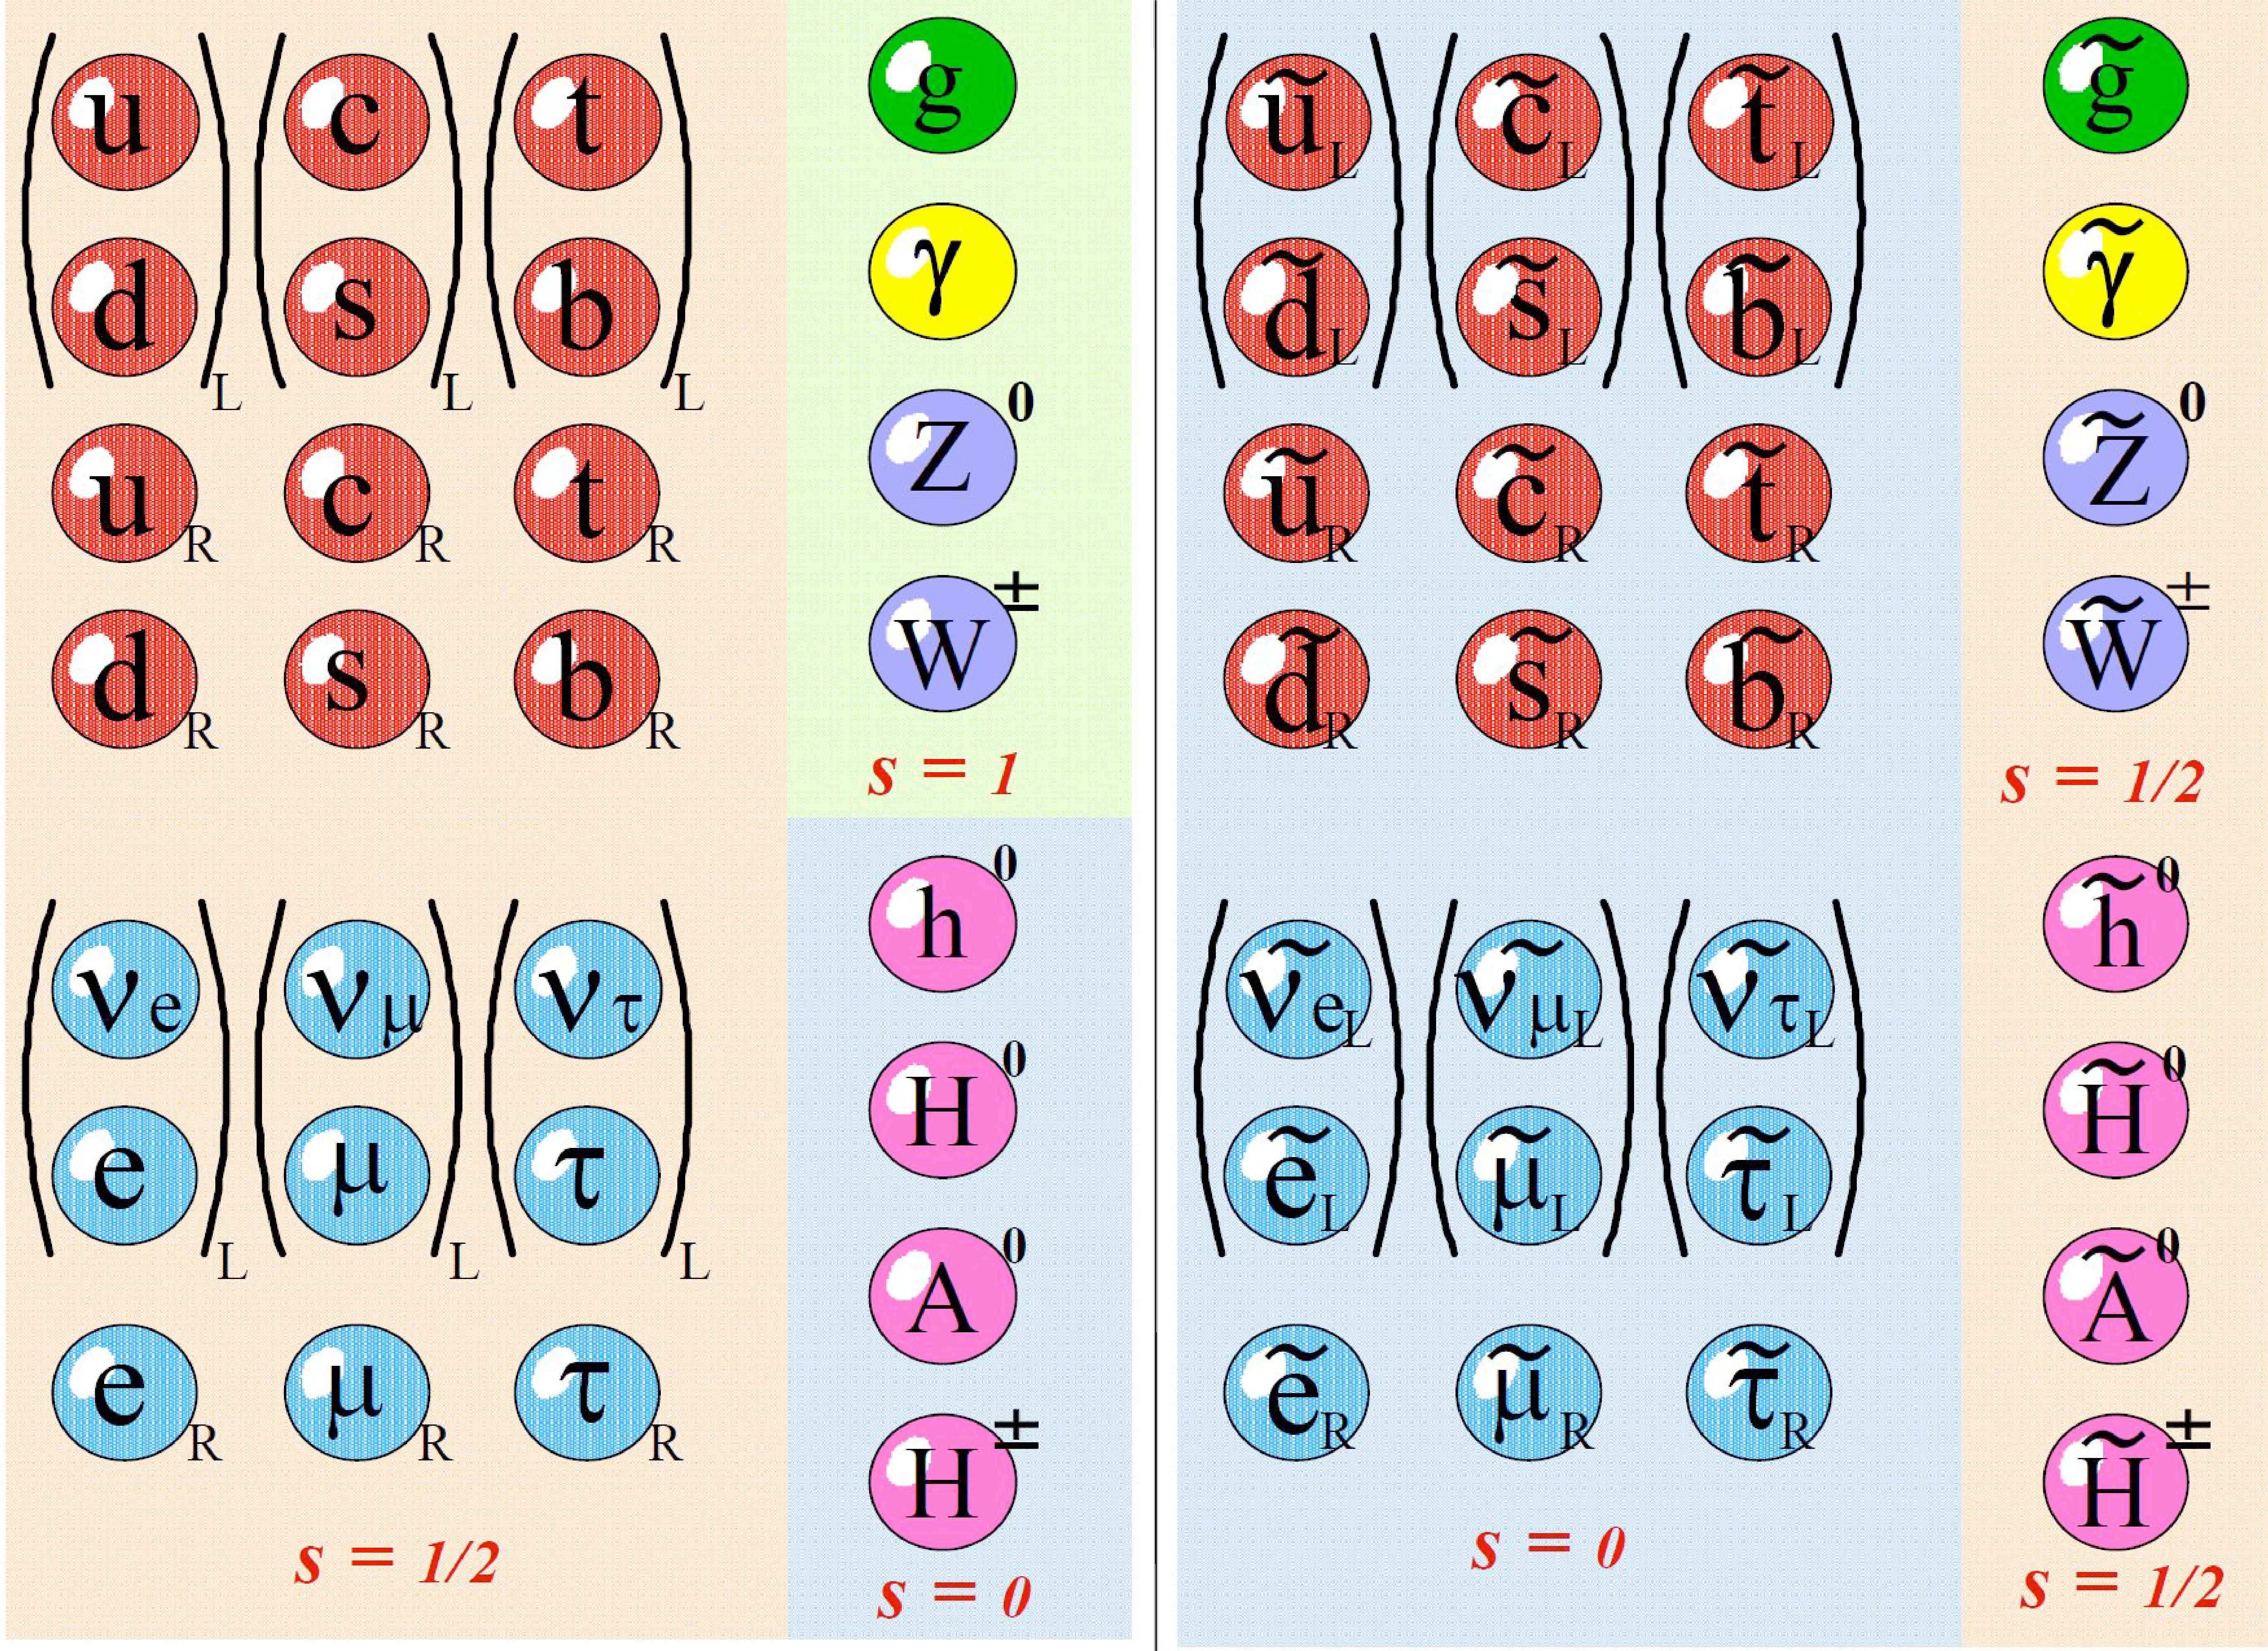
\includegraphics[width=0.98\textwidth]{figs/theory/SMtoSUSYparticleContent.png}
  \end{center}
  \caption[Particle content of the minimal supersymmetric standard model]{Particle content of the minimal supersymmetric standard model~\cite{KEK:2012}.}
  \label{fig:theory:particlesSUSY}
\end{figure}

We can now note how SUSY can address some of the unanswered questions in physics we listed in the beginning of this section.
One of which it can explicitly address is known as the Hierarchy Problem, or as I put it before, ``why is the Higgs so light.''
The problem can be stated as follows: if the standard model is valid all the way up to the Planck scale, would expect the mass of the Higgs, due to the perturbative loop corrections seen in Figure~\ref{fig:theory:HiggsMassLoops}, to be on the order of the Planck scale.
We of course do not see this with the observed mass of 125~\GeV of a SM like Higgs.
\begin{figure}[ht]
  \begin{center}
    \includegraphics[width=0.98\textwidth]{figs/theory/HiigsMassLoops.png}
  \end{center}
  \caption{The observed Higgs mass as a sum of the bare Higgs mass plus loop corrections.}
  \label{fig:theory:HiggsMassLoops}
\end{figure}
With the addition of superparters we find that a delicate cancellation occurs, where large loop corrections to the Higgs mass existed coming from the top quark ($t$) mass are now canceled by loop corrections arising from the stop quark ($\tilde t$) as is illustrated in Figure~\ref{fig:theory:HiggsMassLoopsSUSY}.
Now, in order for the MSSM to solve the hierarchy problem in this way, we expect the characteristic mass scale of the supersymmetry breaking sector to be on the order of $m_{soft}$ = 1~\TeV.
Therefore, it is reasonable to expect that masses of the few lightest sparticles are approximately at the \TeV scale and are potentially reachable at the LHC!
\begin{figure}[ht]
  \begin{center}
    \includegraphics[width=0.98\textwidth]{figs/theory/HiigsMassLoopsSUSY.png}
  \end{center}
  \caption{The observed Higgs mass as a sum of the bare Higgs mass plus loop corrections now including contributions from SUSY particles. The large blue ``$\textcolor{blue}{+}$'' sign from the stop loop illustrating the it's effective cancellation with the top loop contribution with the red ``$\textcolor{red}{-}$'' sign.}
  \label{fig:theory:HiggsMassLoopsSUSY}
\end{figure}

\subsection{\emph{R}-parity}
%\textcolor{red}{\hrulefill \textsc{Unfinished Section}\hrulefill}\\
Within the framework of the MSSM it is now possible to construct terms in the Lagrangian that violate Baryon ($B$) and Lepton number ($L$) to the tune that the proton would decay in approximately $10^{-2}$ seconds (for $\mathcal{O}(1)$ \emph{R}-parity violating couplings, or if minimal flavor violation is assumed the lifetime can be extended to 1 year).
We know of course that the proton does not rapidly decay (with lifetime bounds currently at $6\times10^{39}$ years) and we also do not observe lepton number violation, so this problem must be addressed in the theory.
A popular solution is to add in a discrete symmetry known as ``\emph{R}-parity,'' defined as the following,
\begin{equation}
    \text{\emph{P}}_{R}=(-1)^{3(B-L)+2S} 
\end{equation}
Where $S$ is the spin of the particle.
When \emph{R}-parity is conserved at a vertex this forbids $B$ and $L$ violation entirely.
This seems like a pretty reasonable thing to do, as $B$ and $L$ seem to be pretty much conserved as far as we can tell.
Also this \emph{R}-parity conserving solution (RPC) necessarily demands that the Lightest Supersymmetric Particle (LSP) be stable\footnote{R=parity is also a measure for SUSYness, i.e. SUSY particles will always have $P_{R}=-1$ while SM particles will have $P_{R}=+1$}, which would give us a very convenient dark matter candidate.
While this discrete symmetry does indeed accomplish its purpose, \emph{R}-parity is, from a theoretical viewpoint, completely ad hoc, without any fundamental justification.




 



\section{The $B-L$ Minimal Supersymmetric Standard Model} \label{sec:susybminusl}
%\textcolor{red}{\hrulefill \textsc{Unfinished Section}\hrulefill}  \\
An alternative solution is obtained by simply postulating that the MSSM should be extended by a gauged $U(1)_{B-L}$ symmetry (of which \emph{R}-parity is a discrete subgroup) which is spontaneously broken at some scale.
This breaks $L$ and, hence, \BL symmetry.
However, $B$ remains unbroken and therefore proton decay continues to be suppressed below its present experimental bounds.
However, the parameters of the \BL MSSM must still be chosen so as to adequately suppress lepton number violating processes.
This reproduces the exact MSSM particle spectrum with an additional three right handed neutrino chiral multiplets as well as a $Z'_{B-L}$ (and its superpartner) from the broken symmetry.
Below the scale of both spontaneous \BL and SUSY breaking, the observable sector of this theory contains precisely the particle spectrum and gauge group of the Standard Model.
This is known as the \BL Minimal Supersymmetric Standard Model as described from the ``bottom-up'' approach.
Also note that a ``top-down'' approach was shown to be possible in a series of papers \cite{Ambroso:2009sc,Ambroso:2010pe,Braun:2005nv,Ovrut:2014rba,Ovrut:2012wg,Ovrut:2015uea,Ambroso:2009jd} where this exact \BL MSSM is recovered as the low energy theory of heterotic superstring/M-theory.
The continuous $U(1)_{B-L}$ symmetry arising naturally as a consequence of the compactification of heterotic M-theory, which has long been known in a non-supersymmetric context to be the minimal extra gauging of the standard model that remains quantum mechanically anomaly free~\cite{Dumitru:2018jyb}.
That is, the gauged $U(1)_{B-L}$ that arises in this context gives a ``natural way'' to suppress unwanted baryon and lepton number violating decays.
For all of these reasons, \emph{the \BL MSSM appears to be the simplest possible phenomenologically realistic theory of heterotic superstring/M-theory; being exactly the MSSM with right-handed
neutrino chiral supermultiplets and spontaneously broken R-parity}~\cite{Dumitru:2018nct}
The post-EWKSB particle content of the \BL MSSM is illustrated in Figure~\ref{fig:theory:particlesSUSYBL}. 
\begin{figure}[htb]
  \begin{center}
    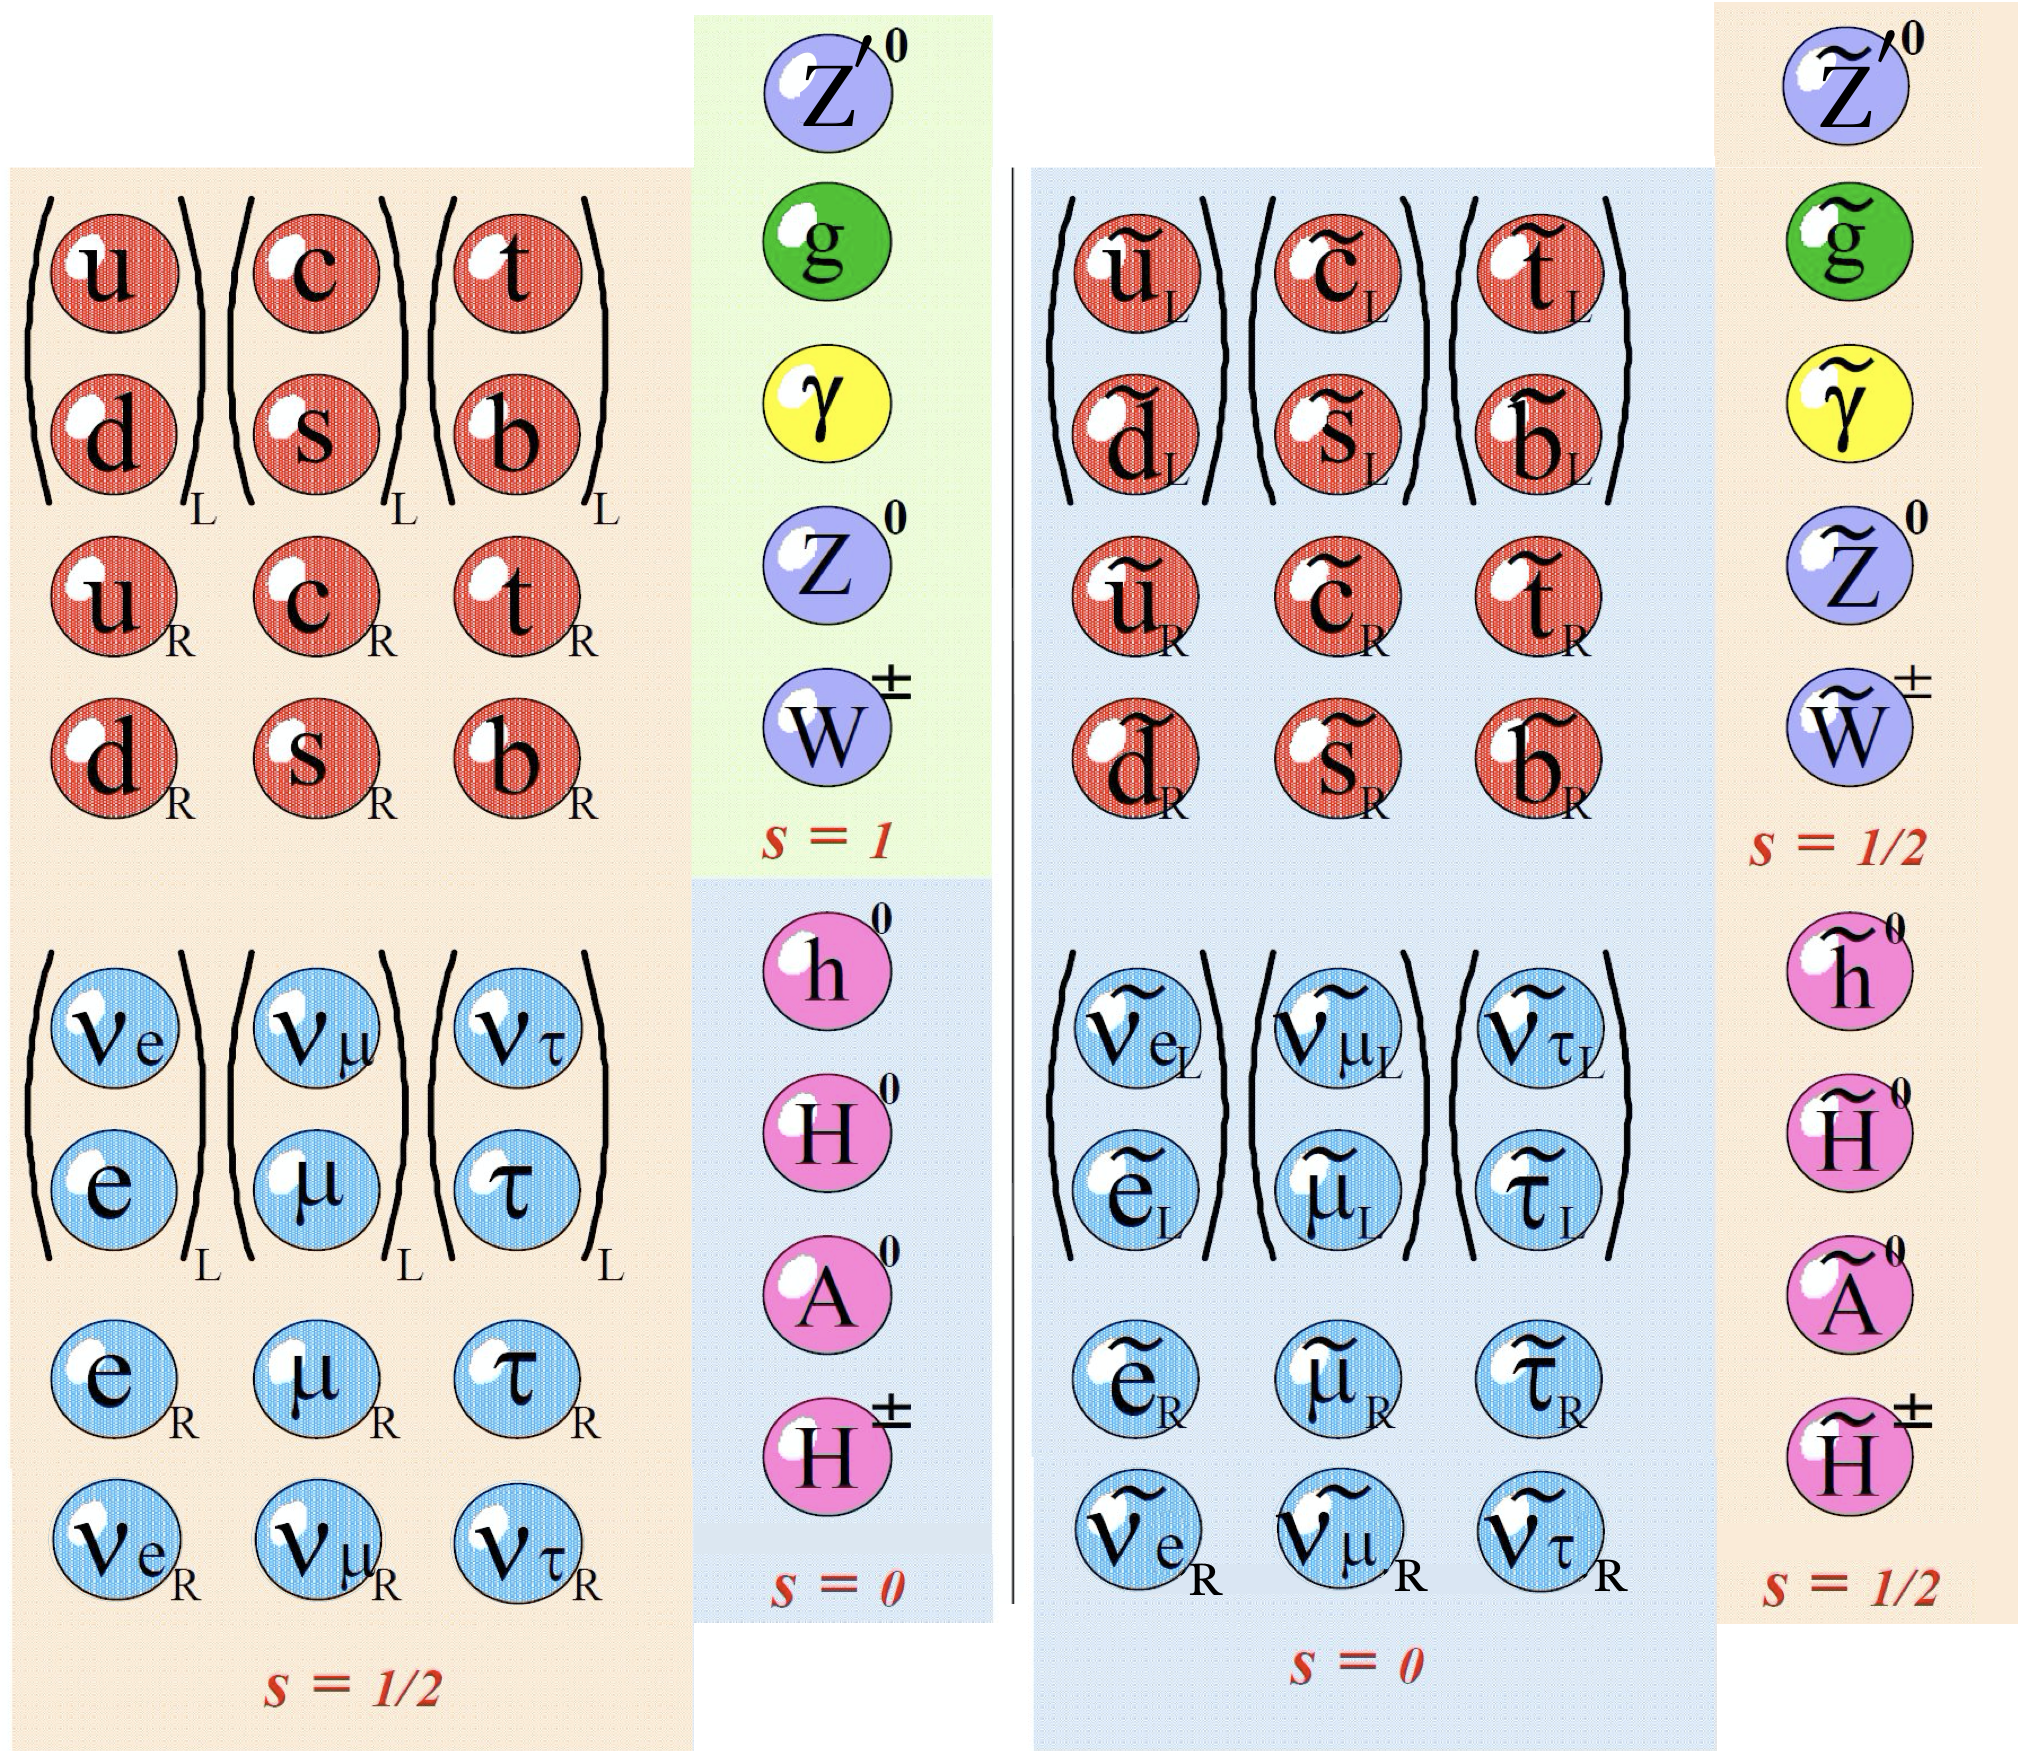
\includegraphics[width=0.98\textwidth]{figs/theory/SMtoBLSUSYparticleContent.png}
  \end{center}
  \caption[Minimal SUSY \BL Model particle content]{The post-EWKSB particle content of the \BL MSSM.
  Referring back to Figure~\ref{fig:theory:particlesSUSY} we note the addition of both right-handed neutrinos and sneutrinos. 
  A $Z'$ and its superpartner coming from the broken $U(1)_{B-L}$ symmetry are also added~\cite{KEK:2021}}
  \label{fig:theory:particlesSUSYBL}
\end{figure}
The gauge group for the \BL MSSM is then
\begin{equation}
    SU(3)_{C} \times SU(2)_{L} \times U(1)_{Y} \times U(1)_{B-L}
\end{equation}
However, as discussed in detail in~\cite{Ovrut:2012wg}, it is equivalent and convenient to choose the gauge group to be
\begin{equation}
    SU(3)_{C} \times SU(2)_{L} \times U(1)_{3R} \times U(1)_{B-L}
\end{equation}
where $U(1)_{3R}$ is the canonical Abelian subgroup of $SU(2)_{R}$.
It was shown in~\cite{Ovrut:2012wg} that there is no kinetic mixing between the field strengths of $U(1)_{3R}$ and $U(1)_{B-L}$ at any momentum scale, and that this is the unique basis with this property.
This vastly simplifies the solution of the RGEs and therefore the analyses done in the cited works work in this gauge group and so as to remain consistent the literature we will as well.
The particle content corresponding to this gauge group is illustrated in Figure~\ref{fig:theory:particlesSUSYBLpreB-LSB}.
\begin{figure}[tb]
  \begin{center}
    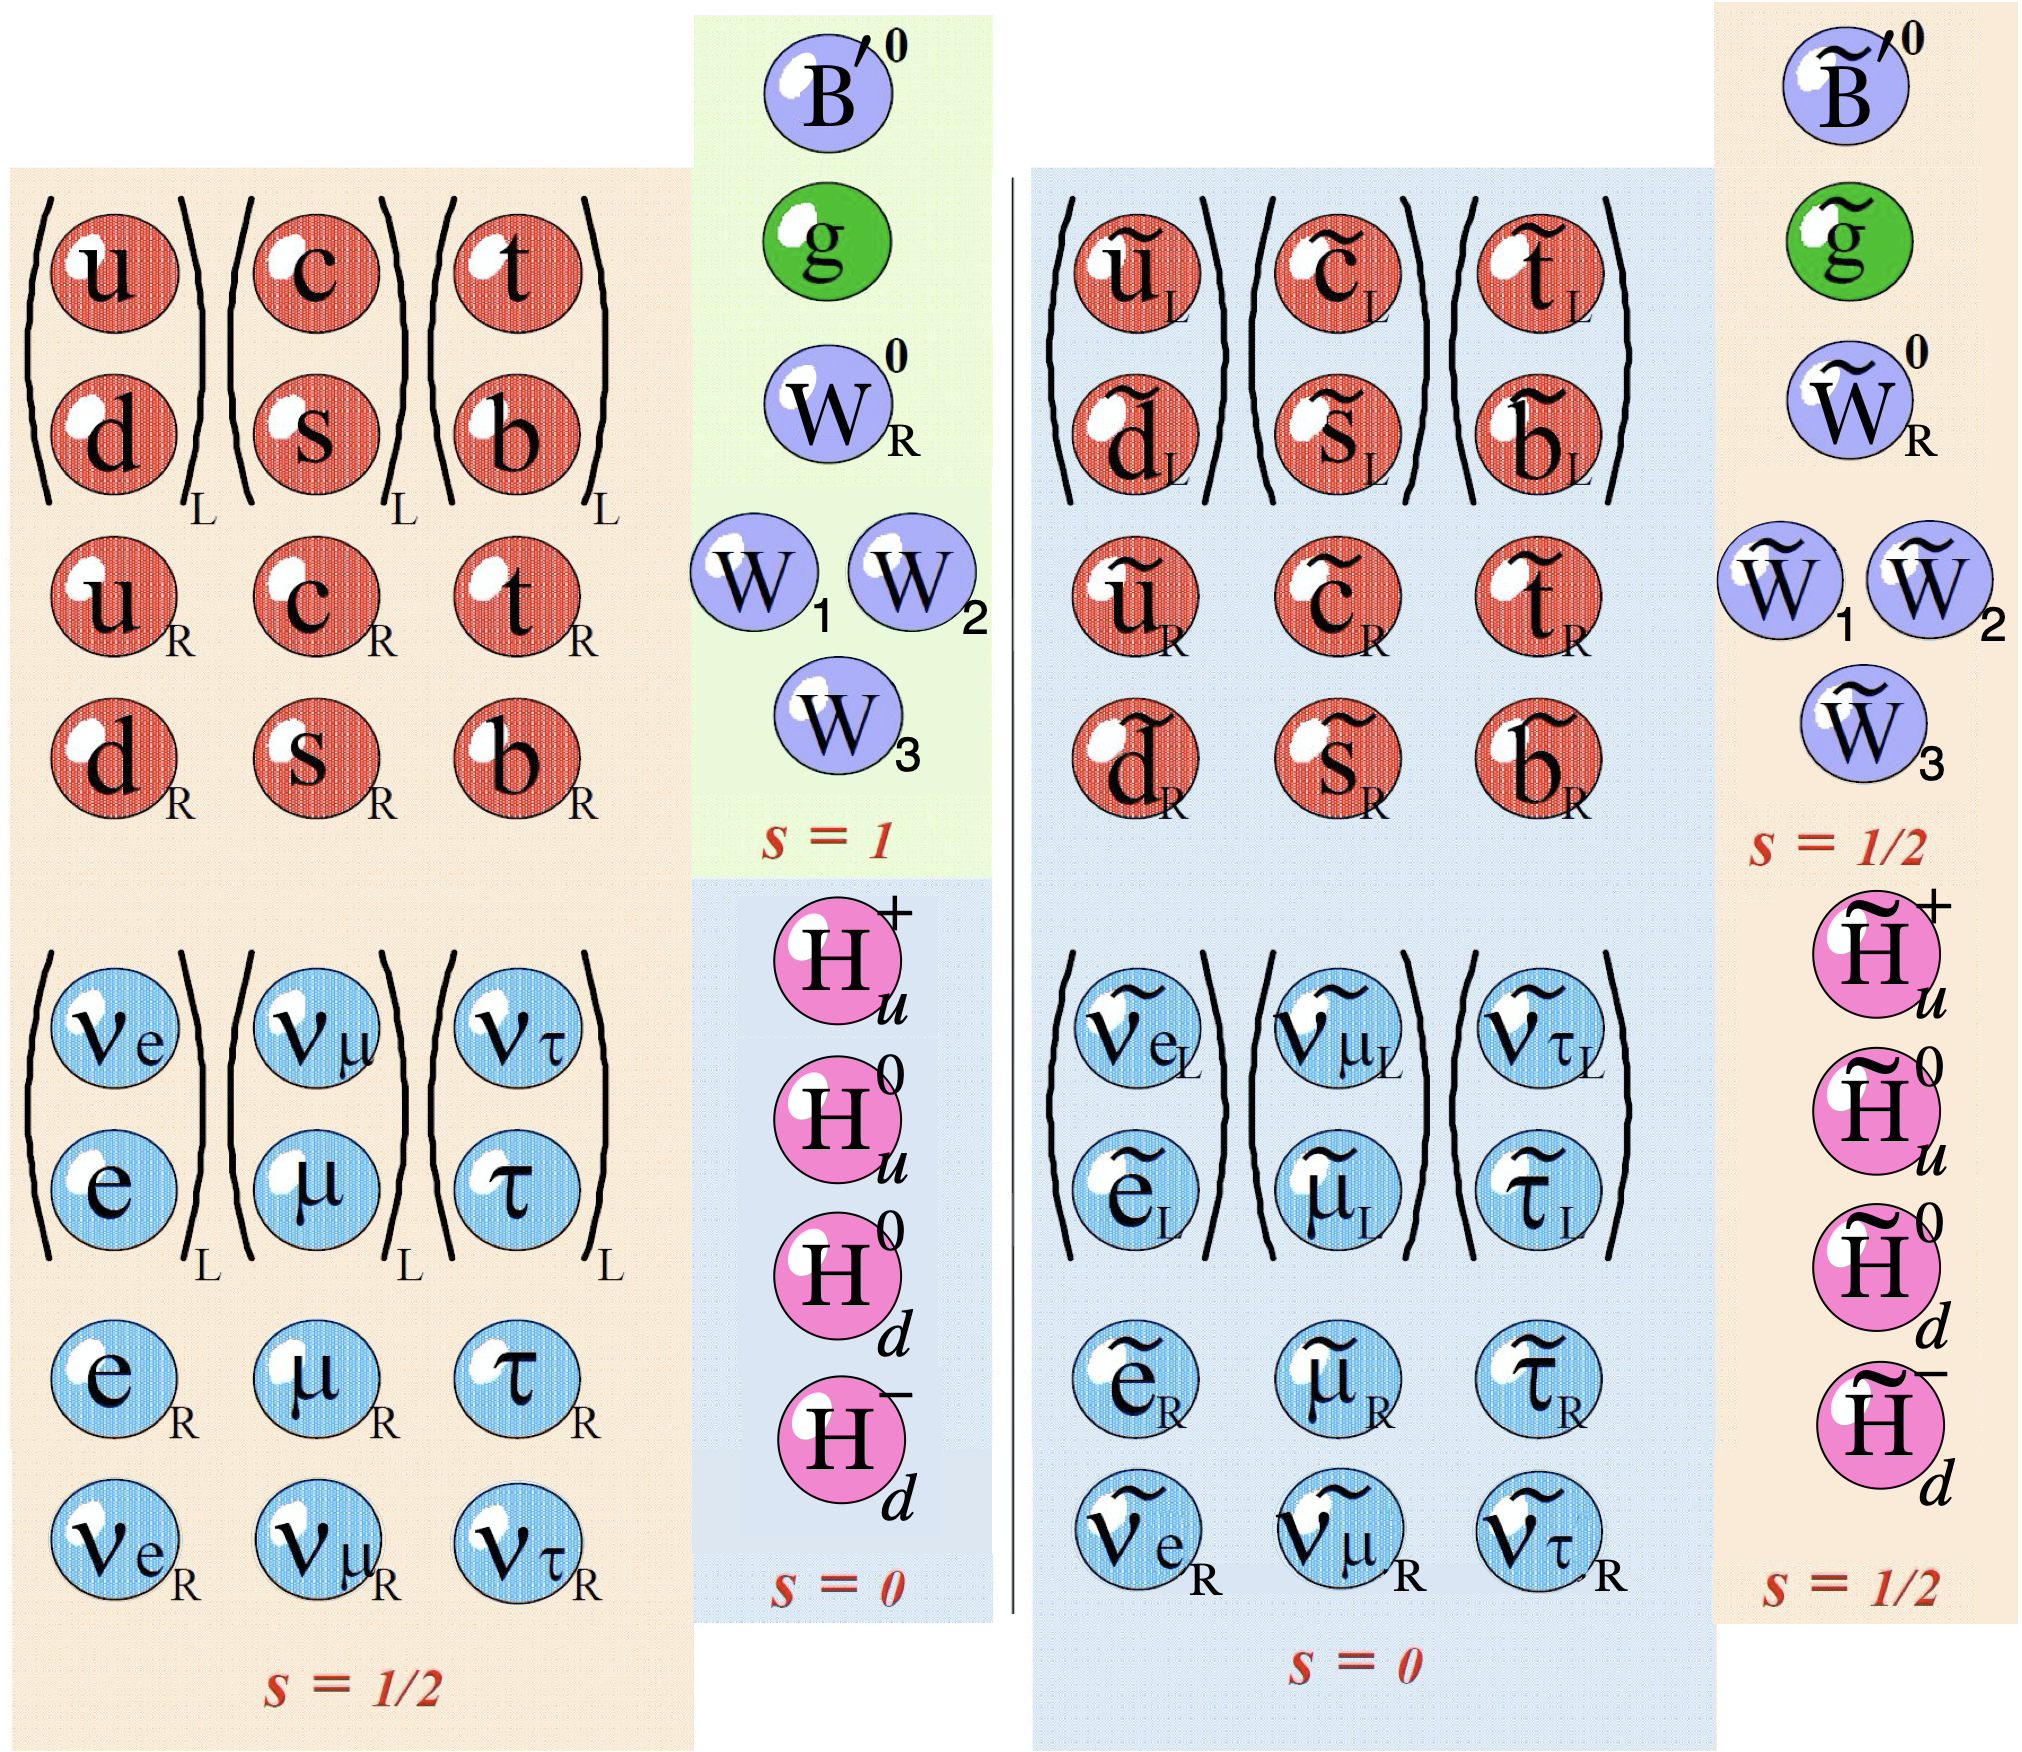
\includegraphics[width=0.98\textwidth]{figs/theory/ParticlesRPVSUSYpreB-LSB.png}
  \end{center}
  \caption[Minimal SUSY \BL Model particle content, pre-\BL breaking]{\cite{KEK:2021}}
  \label{fig:theory:particlesSUSYBLpreB-LSB}
\end{figure}
Note the Blino ($B'^{0}$) and Rhino ($W_{R}^{0}$), corresponding to $U(1)_{B-L}$ and $U(1)_{3R}$ gauge symmetries respectively, in the Figure. 

\subsection{Phenomenology of a Broken $B-L$ Symmetry}
In this theory the $U(1)_{B-L}$ symmetry can in principle be spontaneously broken by the right-handed sneutrino acquiring an non-vanishing vacuum expectation value (VEV).
It was proven that this VEV could dynamically occur via radiative breaking in the \BL MSSM using a full renormalization group (RG) analysis in~\cite{Ambroso:2009jd}.
Of course, the symmetry must be spontaneously broken at a scale sufficiently high to account for the fact that its associated massive vector boson $Z'_{B-L}$ has, so far, not been observed.

A consequence of the breaking of $U(1)_{B-L}$ is the introduction of \emph{R}-Parity violating terms, which will not significantly affect the mass eigenstates, \emph{but do introduce mixing between the gauginos and the standard model charged leptons}~\cite{Dumitru:2018jyb}.
These mixings are central to this thesis as these are what allow for RPV decays and result in interesting signatures not well covered by standard SUSY searches at collider experiments.
%is that the superpartners of the charged Higgs, charged \Wboson bosons, and SM charged leptons now mix.
Continuing to work in the $SU(3)_{C} \times SU(2)_{L} \times U(1)_{3R} \times U(1)_{B-L}$ basis, the charged\footnote{electromagnetically} mixed mass eigenstates, called \emph{charginos}, are related to the gauge eigenstates by unitary matrices $\mathcal{V}$ and $\mathcal{U}$ defined by 
%We also note that making N = 1 (MSSM) SUSY a local symmetry produces gravitation as the associated gauge field, although in the form of a gravity supermultiplet containing the gravitino as well as the graviton~\cite{Dumitru:2018jyb}.
%That is, the existence of N = 1 supersymmetry puts gravity on par with the strong, weak and electromagnetic gauge interactions~\cite{Dumitru:2018jyb}.
\begin{align}
    \begin{pmatrix}
       \tilde\chi_{1}^{-} \\
       \tilde\chi_{2}^{-} \\
       \tilde\chi_{3}^{-} \\
       \tilde\chi_{4}^{-} \\
       \tilde\chi_{5}^{-} 
    \end{pmatrix}
    =\mathcal{U} 
    \begin{pmatrix}
      \tilde W^{-}\\ 
      \tilde H_{d}^{-}\\ 
      e^{-} \\ 
      \mu^{-} \\ 
      \tau^{-} 
    \end{pmatrix},\hspace{1.0cm}
    \begin{pmatrix}
       \tilde\chi_{1}^{+} \\
       \tilde\chi_{2}^{+} \\
       \tilde\chi_{3}^{+} \\
       \tilde\chi_{4}^{+} \\
       \tilde\chi_{5}^{+} 
    \end{pmatrix}
    =\mathcal{V} 
    \begin{pmatrix}
      \tilde W^{+} \\ 
      \tilde H_{u}^{+} \\ 
      e^{+} \\ 
      \mu^{+} \\ 
      \tau^{+} 
    \end{pmatrix}
\end{align}
Where the explicit values for the entries in  $\mathcal{V}$ and $\mathcal{U}$ can be found in~\cite{Dumitru:2018jyb}.
For the analogous neutral mass eigenstates, \emph{neutralinos}, we have an even more complicated situation.
First, it has been shown that mixing with the first- and second-family right-handed neutrino would lead to active sterile neutrino oscillations~\cite{Dumitru:2018jyb}.
Unless and until there is more experimental evidence of such oscillations, we will assume that they do not exist. 
Therefore, the mixing with the first and second-family right-handed neutrinos is negligible and we include only mixing with the three families of left-handed neutrinos and the third-family right-handed neutrino~\cite{Dumitru:2018jyb}.
The neutralinos are then related to the gauge eigenstates by unitary matrix $\mathcal{N}$ defined by
\begin{align}
    \begin{pmatrix}
       \tilde\chi_{1}^{0} \\
       \tilde\chi_{2}^{0} \\
       \tilde\chi_{3}^{0} \\
       \tilde\chi_{4}^{0} \\
       \tilde\chi_{5}^{0} \\
       \tilde\chi_{5}^{0} \\
       \tilde\chi_{5}^{0} \\
       \tilde\chi_{5}^{0} \\
       \tilde\chi_{5}^{0} 
    \end{pmatrix}
    =\mathcal{N} 
    \begin{pmatrix}
      \tilde W_{R}\\ 
      \tilde W^{0}\\ 
      \tilde H_{d}^{0}\\ 
      \tilde H_{u}^{0}\\ 
      \tilde B'\\ 
      \nu_{3}^{c}\\
      \nu_{e}\\
      \nu_{\mu}\\
      \nu_{\tau}
    \end{pmatrix}
\end{align}
Where again the explicit values for the entries in  $\mathcal{N}$ can be found in~\cite{Dumitru:2018jyb}.
Now due to the relative smallness of the RPV couplings we expect RPV decays primarily coming from the LSP of the theory, as heavier charginos/neutralinos would prefer RPC decay channels.
So it then becomes important to determine if the \chono\footnote{The lightest chargino and neutralino state respectively} are even likely candidates to be the LSP in the \BL MSSM. 
An extensive study involving the statistical scanning over all dimensionful parameters of the soft SUSY breaking terms was done in \cite{Dumitru:2018jyb} and does motivate \chono  as likely LSPs in the \BL MSSM.
This scan is discussed in more detail in Chapter~\ref{ch:rpvthreel} where additional experimental considerations are taken into account as well.


%\begin{figure}[htb]
%  \begin{center}
%    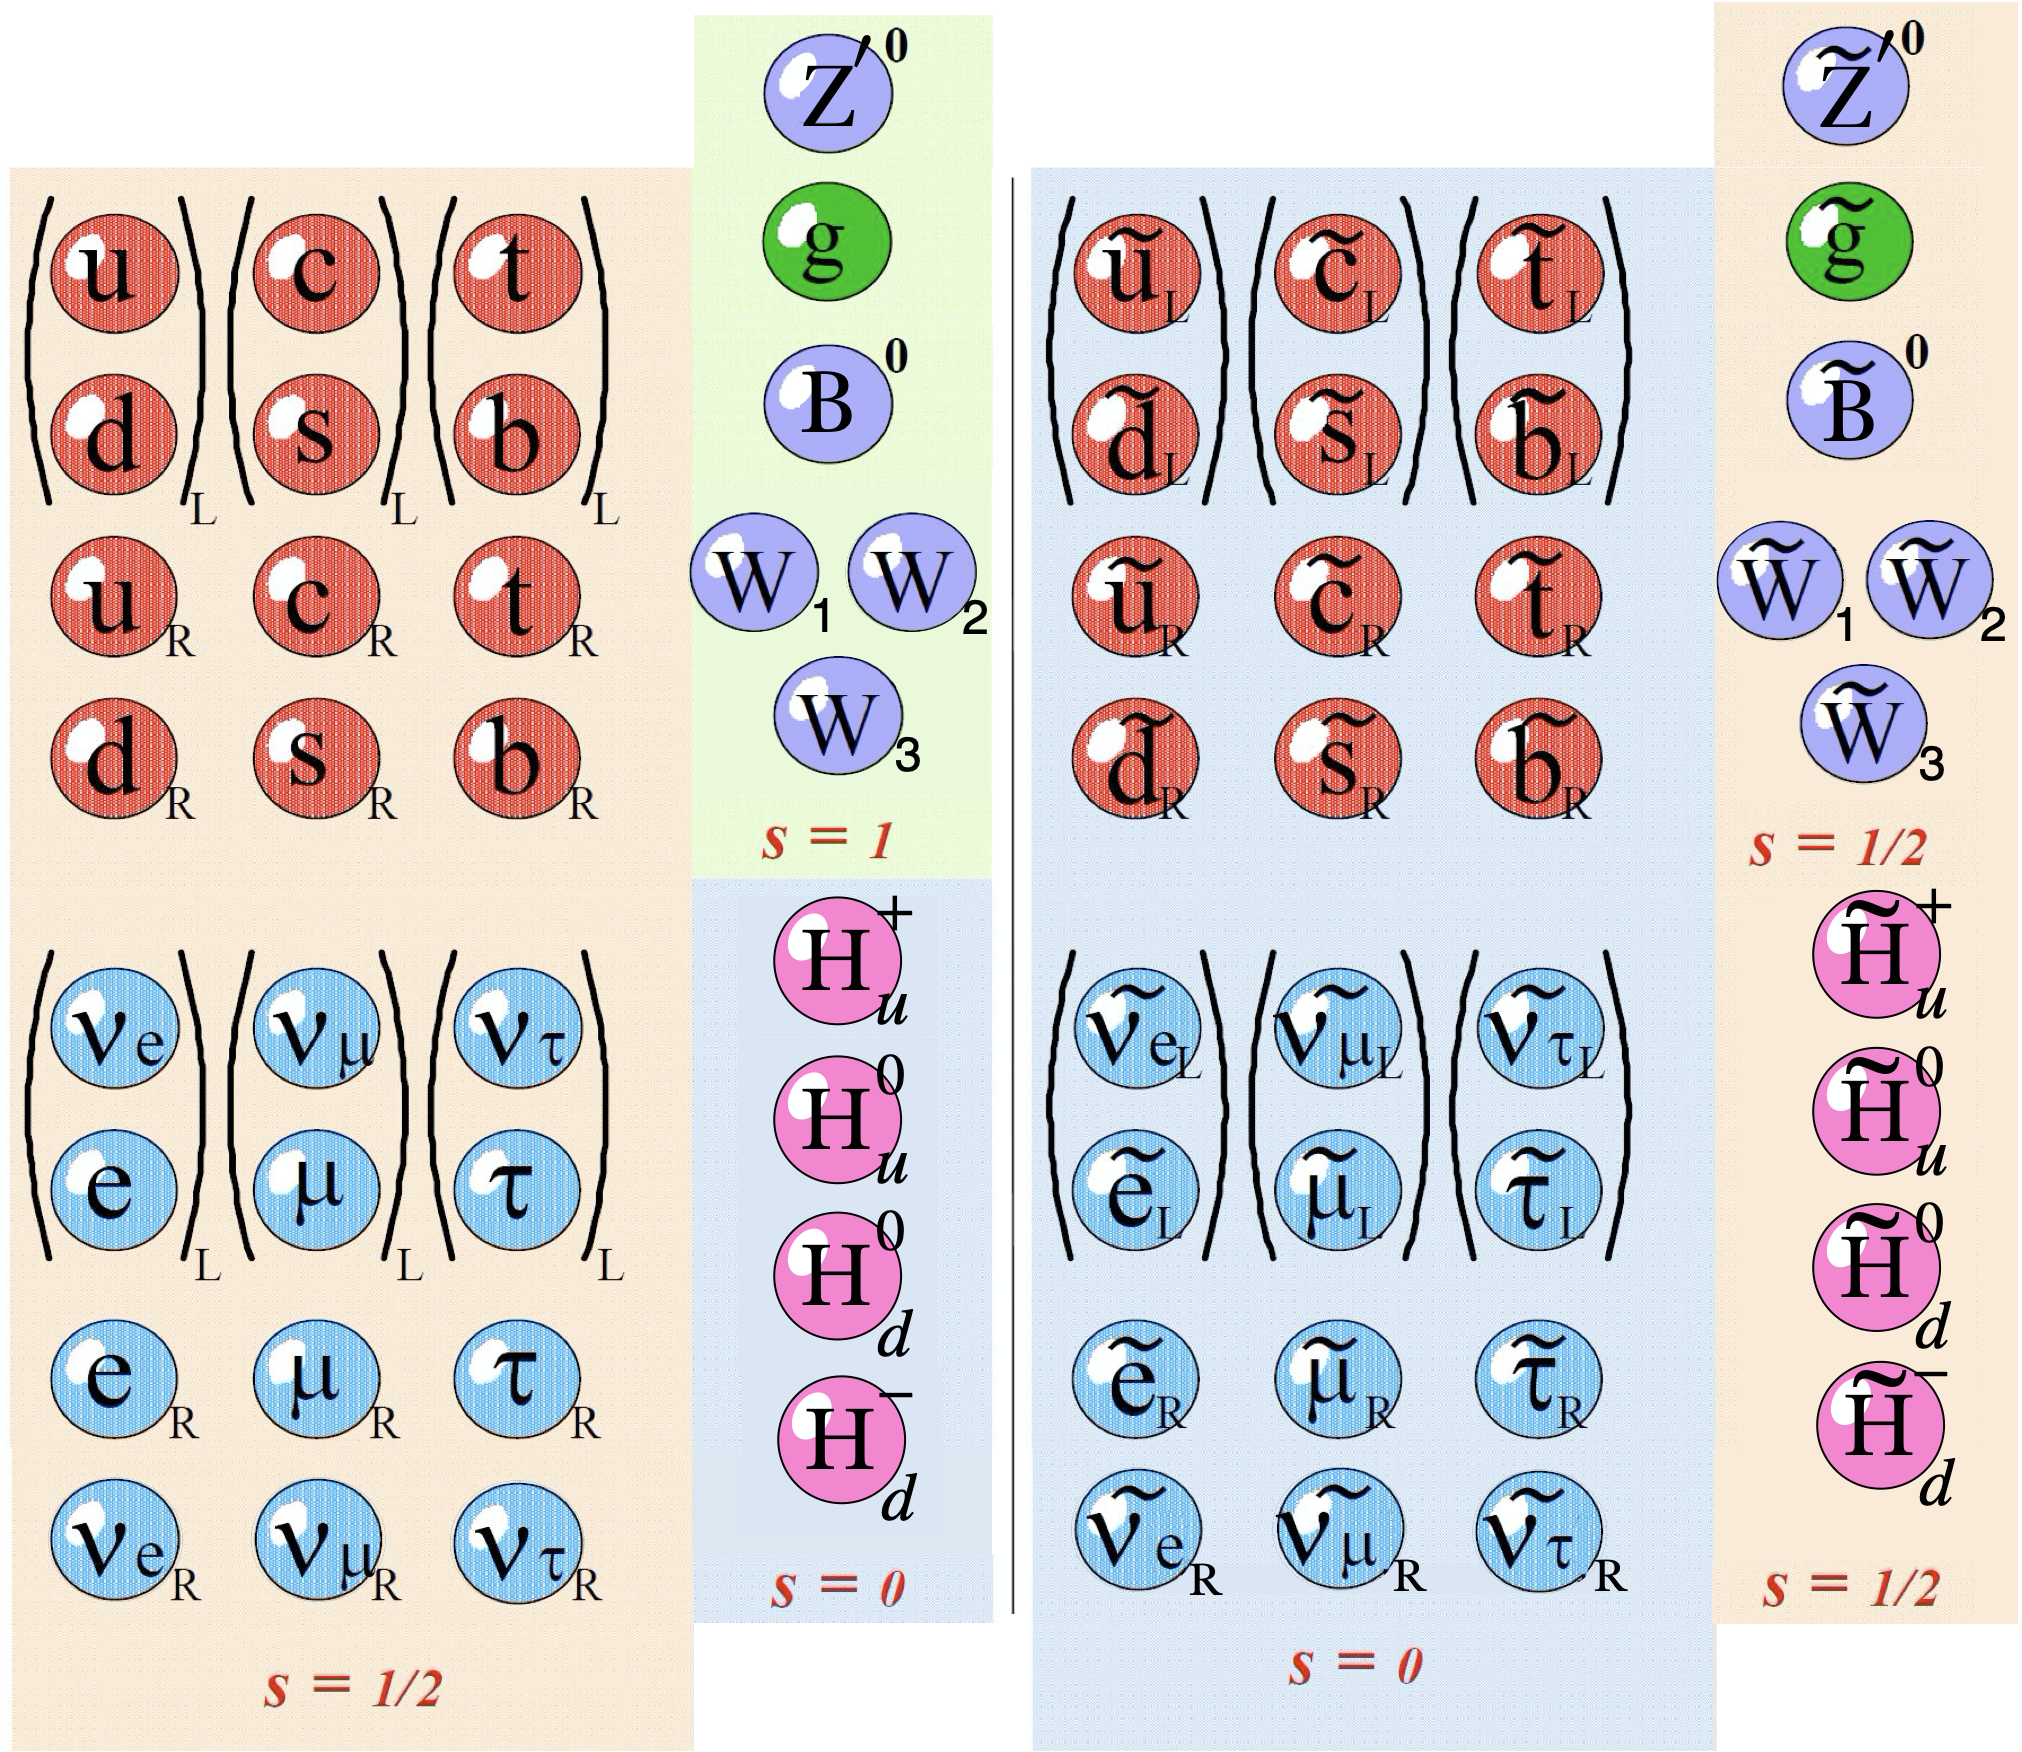
\includegraphics[width=0.98\textwidth]{figs/theory/ParticlesRPVSUSYpreEWKSB.png}
%  \end{center}
%  \caption[Minimal SUSY \BL Model particle content, pre-EWKSM]{\cite{KEK:2021}}
%  \label{fig:theory:particlesSUSYBLpreEWKSB}
%\end{figure}

%It is important to note that despite the violation of \emph{R}-parity, an LSP gravitino can live long enough to potentially play the role of dark matter~\cite{Buchmuller:2007ui,Takayama:2000uz}.

